
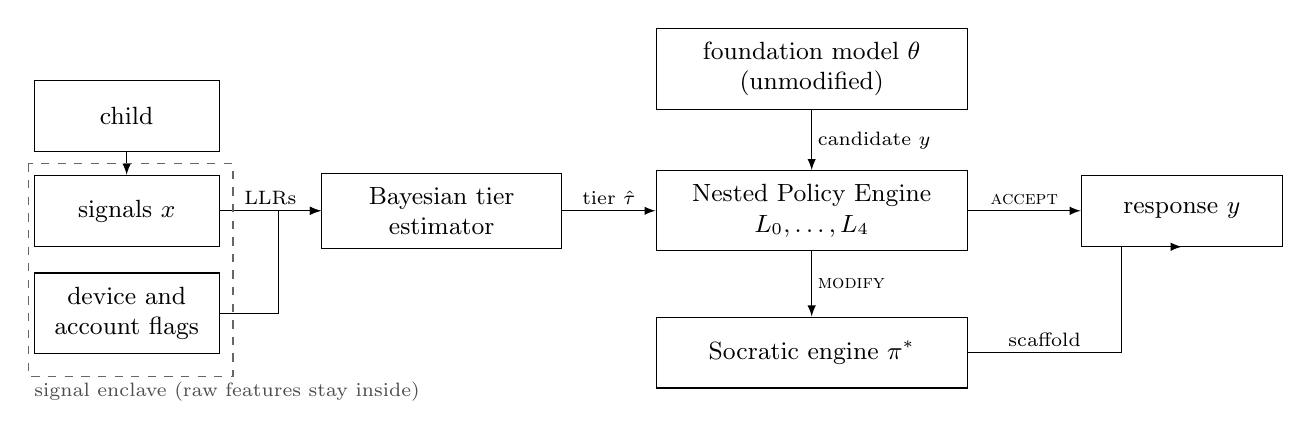
\begin{tikzpicture}[
  box/.style={draw, thin, rectangle, align=center, inner sep=5pt,
              minimum height=9mm, font=\small},
  ar/.style={-latex, thin},
  obs/.style={-latex, thin, dashed},
  lab/.style={font=\scriptsize, inner sep=2pt},
]
\node[box, text width=20mm] (c)  at (0.7,1.55) {child};
\node[box, text width=20mm] (s)  at (0.7,0.35) {signals $x$};
\node[box, text width=20mm] (dv) at (0.7,-0.95) {device and\\account flags};

\node[box, text width=27mm] (est) at (4.7,0.35) {Bayesian tier\\estimator};
\node[box, text width=36mm] (pol) at (9.4,0.35) {Nested Policy Engine\\$L_0,\ldots,L_4$};
\node[box, text width=36mm] (llm) at (9.4,2.15) {foundation model $\theta$\\(unmodified)};
\node[box, text width=36mm] (soc) at (9.4,-1.45) {Socratic engine $\pi^{*}$};
\node[box, text width=22mm] (out) at (14.1,0.35) {response $y$};

\draw[ar] (c) -- (s);
\draw[ar] (s) -- node[lab, above] {LLRs} (est);
\draw[ar] (dv.east) -- ++(0.75,0) |- (est.west);
\draw[ar] (est) -- node[lab, above] {tier $\hat{\tau}$} (pol);
\draw[ar] (llm) -- node[lab, right] {candidate $y$} (pol);
\draw[ar] (pol) -- node[lab, right] {\textsc{modify}} (soc);
\draw[ar] (pol) -- node[lab, above] {\textsc{accept}} (out);
\draw[ar] (soc.east) -- ++(1.95,0) node[lab, above, pos=0.5] {scaffold} |- (out.south);

% trust boundary around the signal enclave
\draw[dashed, thin, black!60] (-0.55,0.95) rectangle (2.05,-1.75);
\node[lab, anchor=north west, text=black!70] at (-0.55,-1.75) {signal enclave (raw features stay inside)};
\end{tikzpicture}
